\section{Výpočet hustoty stavov Thoulesovým ansatzom}
V tejto kapitole vypočítame hustotu stavov pomocou Thoulesovho ansatzu. Self energiu, narozdiel od AA, nie je možné vyjadriť analyticky, preto použijeme jednoduchú obdĺžnikovú metódu integrovania. Výsledok porovnáme s AA a experimentom. Vychádzame z pre energiu elektronov v kove s disorderom a e-e interakciou \eqref{MISSING_REFERENCE}
\begin{align}
\label{eq:05energy} 
 E_m=\E_m-\sum_{\forall m'} \int d\vr\' \int d\vr \phi_{m'}^*(\vr\')\phi_{m}^*(\vr)V(|\vr-\vr\ '|)\phi_{m'}(\vr)\phi_{m}(\vr\')\text{,}
\end{align} 
kde $\E_m$,$\phi_m$  sú riešenia \eqref{eq:01schr_dis}
\begin{align}
\label{eq:05schr_dis}
[\frac{\hbar^2}{2m}\laplace+V_{dis}(\vr)]\phi_m(\vr)=\E_m\phi_m(\vr)\text{,}
\end{align}
a $V(|\vr -\vr\ '|)$ je Yukkavov potenciál \eqref{eq:01yukk_pot}, resp. jeho Fourierova transformácia
\begin{align}
\label{eq:05yukkft}
V(|\vr - \vr\ '|) &= \frac{1}{(2\pi)^3}\int d\vq\ V(\vq)e^{i|\vr-\vr\ '|\vq} \text{.} \\
\notag
V(\vq)&\equiv\frac{e^2q^2}{\epsilon_0(q^2+k_s^2)} 
\end{align}

Do \eqref{eq:05energy} dosadíme \eqref{eq:05yukkft} za $V(\vr-\vr\ ')$. Pre energiu stredného disorderu dostávame
\begin{align}
\label{eq:05ergmeandis}
\overline{E_m} =\overline{\E_m} - \frac{1}{(2\pi)^3}\int d\vq\ V(q) \sum_{\forall m'}\overline{|\bra{\phi_m}e^{i\vq\vr}\ket{\phi_{m'}}|}
\end{align}

Vlnovú funkciu $\phi_m(\vr)$ rozvinieme do systému rovinných vĺn
\begin{align}
\label{eq:05phi}
\phi_m(\vr) = \frac{1}{\sqrt{\Omega}}\sum_{\vk}c_{\vk}^me^{i\vk\vr}\text{,}
\end{align}
a dosadíme do \eqref{eq:05ergmeandis}
\begin{align}
\notag
\overline{E_m} = \E_m - \frac{1}{(2\pi)^3}&\int d\vq\ V(\vq)\overline{ \sum_{m'} \sum_{\vk_1} \sum_{\vk_3}\int d\vr c^{m*}_{\vk_1}c^{m'}_{\vk_3}e^{i\vq\vr}e^{i\vk_1\vr}e^{-i\vk_3\vr}}\\
&\overline{\sum_{\vk_2}\sum_{\vk_4}\int d\vr\' c^{m'*}_{\vk_4}c^{m}_{\vk_2}e^{-i\vq\vr\ '}e^{-i\vk_4\vr\ '}e^{i\vk_2\vr\ '}} \text{.}
\end{align}
Podobne ako v kapitole \ref{sec:kubo} pre vzťah \eqref{eq:03dfisquared} vieme využiť nasledovné vzťahy
Využijeme nasledovné vzťahy:
\begin{align*}
\int d\vr\ e^{i(\vk+\vq-\vk)\vr}=\delta(\vk_3-\vk_1-\vq)
\int d\vr\ e^{i(\vk_2+\vq-\vk_4)\vr}=\delta(\vk_3-\vk_1-\vq)
\end{align*}
Vysumujeme cez Kroneckerove symboly, a dostaneme
\begin{align}
\overline{E_m}=\overline{\E_m} - \frac{1}{(2\pi)^3}\int d\vq V(\vq) \sum_{m'}\sum_{\vk}\sum_{\vk\ '}\overline{c^{*m}_{\vk+\vq}c^{m}_{\vk\ '+\vq}c^{*m'}_{\vk\ '}c^{m'}_{\vk}}\text{.}
\end{align}
Uvažujeme {\it slabý} disorder, koeficienty s rôznym $m$ a s rôznym $\vk$ sú nekorelované  - viď. kapitolu \ref{sec:kubo}, kde sme urobili to isté pri prechode z \eqref{eq:03dfisq2} na \eqref{eq:03dfisq3}. Dostaneme výraz pre energiu
\begin{align}
\label{eq:05energy2}
\overline{E_m}=\overline{\E_m} - \frac{1}{(2\pi)^3} \int d\vq\ V(\vq) \sum_{m'}\sum_{\vk} \overline{c^{m*}_{\vk+\vq}c^{m}_{\vk+\vq}}\ \overline{c^{m*}_{\vk}c^{m}_{\vk}} \text{.}
\end{align}

Teraz môžme aplikovať Thoulessov ansatz:
\begin{align}
\label{eq:05thouless}
\overline{c^{m*}_{\vk}c^{m}_{\vk}}=\frac{1}{\pi \rho(\epsilon_m)}\lorenz{\epsilon_m}
\end{align}
Zavedieme nasledovné označenia
\begin{align*}
\epsilon_\tau &\equiv \frac{\hbar}{2\tau} \\
\epsilon_{|\vk+\vq|}&\equiv\frac{\hbar^2|\vk+vq|^2}{2m}
\end{align*}
%+
Po dosadení Thoulesovho ansatzu \eqref{eq:05thouless} do \eqref{eq:05energy2} dostaneme  

\begin{align}
\label{eq:05energy3}
\overline{E_m}=\overline{\E_m} - \frac{1}{(2\pi)^3} \int d\vq\ V(\vq) \sum_{m'}\sum_{\vk}\frac{1}{\pi\rho(\epsilon_m)}\frac{\epsilon_\tau}{(\epsilon_m-\epsilon_k)^2-\epsilon_\tau^2}\frac{1}{\pi\rho(\epsilon_{m'})}\frac{\epsilon_\tau}{(\epsilon_{m'}-\epsilon_{|\vk+\vq|})^2-\epsilon_\tau^2} \text{.}
\end{align}

Prejdeme od súm cez $m$ a $\vk$ k integrálom cez energie. Zároveň prepíšeme $q$ do sférických súradníc. 
\begin{align}
\label{eq:05energy4}
\notag
\overline{E_m}=\overline{\E_m} - \frac{1}{8\pi^2\rho(\epsilon_m)} \int dq\ q^2 V(q) \int_0^{E_F} d\epsilon_{m'} \\
\int_0^{\infty} \rho(\epsilon_k) d \epsilon_k \int_0^\pi \sin\theta d\theta\ \frac{\epsilon_\tau}{(\epsilon_m-\epsilon_k)^2-\epsilon_\tau^2}\frac{\epsilon_\tau}{(\epsilon_{\vk}+\epsilon_{\vq}+2\sqrt{\epsilon_{\vk}\epsilon_{\vq}}\cos(\theta)-\epsilon_{m'})^2-\epsilon_\tau^2} \text{.} 
\end{align}
Podobne ako v kapitole \ref{sec:thouless}, použijeme aproximáciu $\rho(\epsilon_m)\approx\rho(\epsilon_k)$, čo nám umožňuje vykrátiť dané členy, finálny integrál bude
\begin{align}
\label{eq:05energy5}
\notag
\overline{E_m}=\overline{\E_m} - \frac{1}{8\pi^2} \int dq\ q^2 V(q) \int_0^{E_F} d\epsilon_{m'} \\
\int_0^{\infty} d \epsilon_k  \int_0^\pi \sin\theta d\theta\  \frac{\epsilon_\tau}{(\epsilon_m-\epsilon_k)^2-\epsilon_\tau^2}\frac{\epsilon_\tau}{(\epsilon_{\vk}+\epsilon_{\vq}+2\sqrt{\epsilon_{\vk}\epsilon_{\vq}}\cos(\theta)-\epsilon_{m'})^2-\epsilon_\tau^2} \text{.} 
\end{align}
Integrály cez $d\epsilon_m$ a $d\theta$ vieme vypočítať analyticky. Zvyšné dva budeme musieť rátať numericky, preto zavedieme bezrozmerné premenné:
\begin{align*}
w=\frac{\epsilon_m}{\epsilon_\tau} \\
u=\frac{\epsilon_{m'}}{\epsilon_\tau} \\
x=\frac{\epsilon_k}{\epsilon_\tau} \\
y=\frac{\epsilon_q}{\epsilon_\tau} 
\end{align*}
Po vykonaní oboch analytických integrálov dostaneme vzťah pre selfenergiu
\begin{align}
\label{eq:05selfenergy}
\Sigma(w)=\frac{e^2}{8\pi^4\epsilon_0 k_s^{-1}} \int_0^{\bar y_{max}} d\bar{y}\ \frac{\bar{y}^2}{1+\bar{y}^2}\int_0^{\infty} dx \frac{1}{(x-w)^2+1}\sqrt{\frac{\epsilon_\tau}{E_F}}F(x,y) \text{,}
\end{align}
kde $k_s\approx k_F$ je recipročná tieniaca dĺžka, $\bar{y}=\frac{q}{k_s}$  a $F(x,y)$ je výsledok analytických integrálov
\begin{align*}
F(x,y)=\frac{1}{\sqrt{4xy}}&\{ \\
&(x+y+2\sqrt{xy}-u_{EF})\arctan(x+y+2\sqrt{xy}-u_{EF}) \\
&-(x+y-2\sqrt{xy}-u_{EF})\arctan(x+y-2\sqrt{xy}-u_{EF}) \\
&-(x+y+2\sqrt{xy})\arctan(x+y+2\sqrt{xy}) \\
&+(x+y-2\sqrt{xy})\arctan(x+y-2\sqrt{xy}) \\
&-\frac{1}{2}ln(\frac{(x+y+2\sqrt{xy}-u_{EF})^2+1}{(x+y-2\sqrt{xy}-u_{EF})^2+1}\ \frac{(x+y+2\sqrt{xy})^2+1}{(x+y-2\sqrt{xy})^2+1})\\
&\}\text{,}
\end{align*}
kde $u_{EF}=\frac{E_F}{\epsilon_\tau}$ je normovaná Fermiho Energia.

Numerické riešenie \eqref{eq:05selfenergy} zjednodušíme poslednou aproximáciou. Integrál cez $dx$ môžme považovať za $\delta$ funkciu.
\begin{align}
\delta(x-w)=\int_0^{\infty}dx\ \frac{1}{(x-w)^2+1}
\end{align}
Finálny vzťah pre energiu, ktorý budeme počítať numericky, bude nasledovný
\begin{align}
\label{eq:05selfenergy2}
\Sigma(w)=\frac{e^2}{8\pi^4\epsilon_0 k_s^{-1}} \int_0^{\bar y_{max}} d\bar{y}\ \frac{\bar{y}^2}{1+\bar{y}^2}\sqrt{\frac{\epsilon_\tau}{E_F}}F(w,y) \text{,}
\end{align} 
\begin{figure}
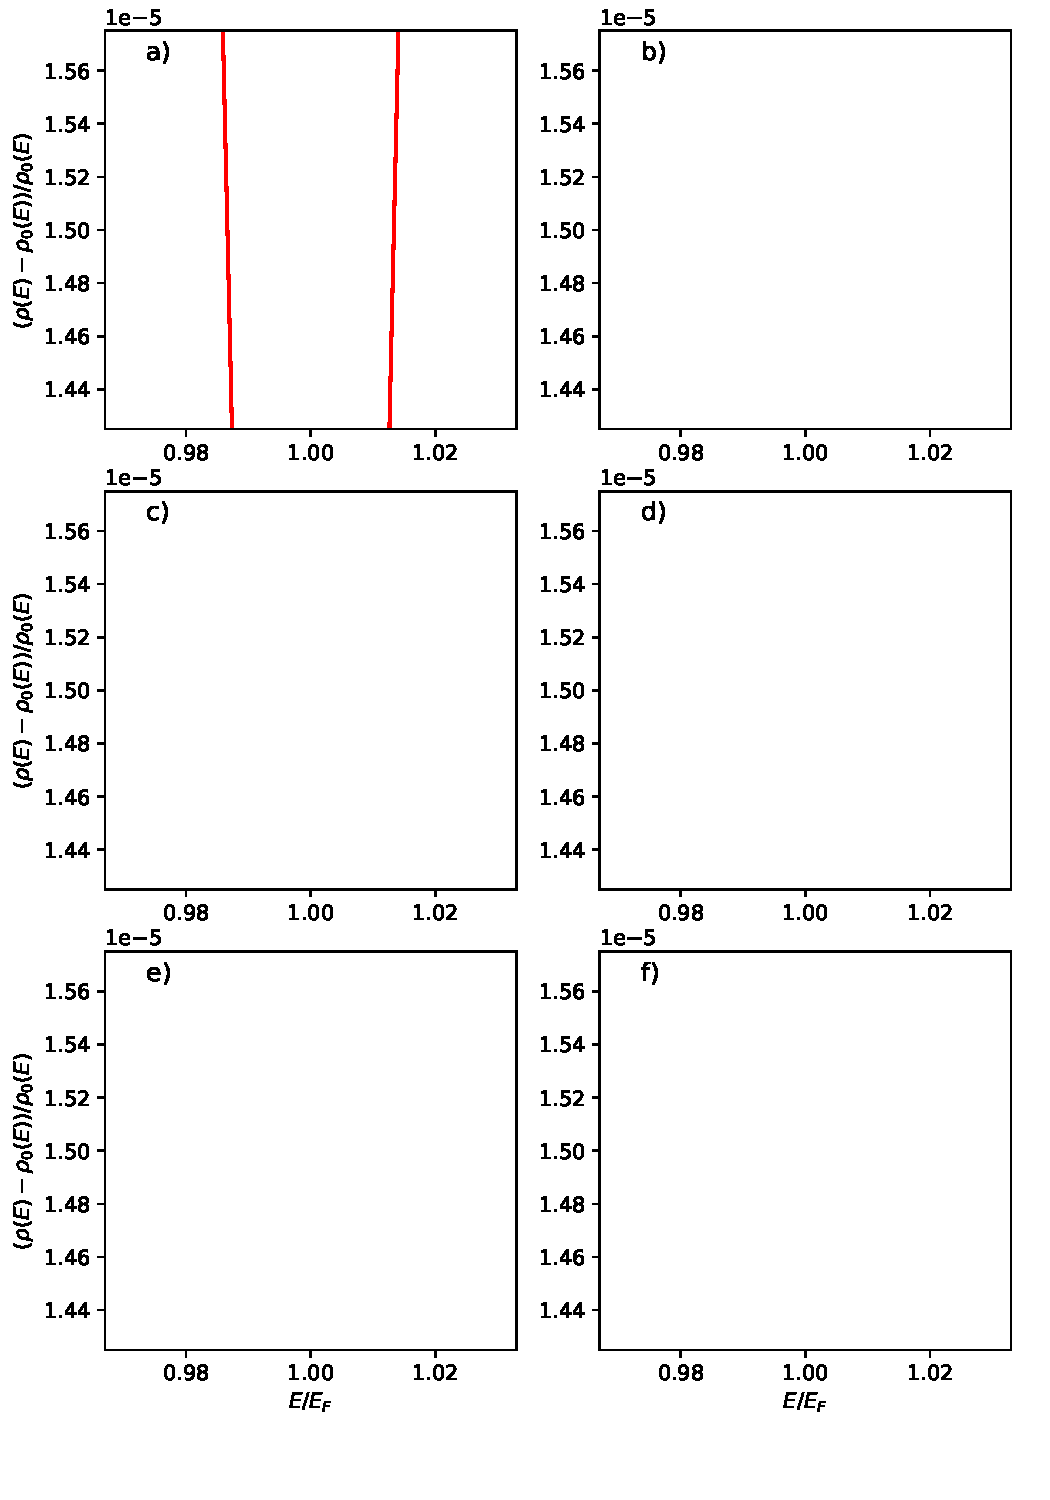
\includegraphics[scale=0.9]{../img/final_data_1k.pdf}
\caption{\lipsum[3]}
\end{figure}